%\section{「印刷する」機能}
印刷する機能はカードリストから画像データや観光情報を取得することによって、1枚のリーフレットを作成する機能である。トップ画面の「印刷する」ボタンをタップするとリーフレットの写真選択画面に遷移する。リーフレットの写真選択画面を図6.7(a)に示す。「タップして写真を選ぶ」と書かれている枠の部分をタップするとリーフレット作成画面に遷移する。リーフレット作成画面に遷移した画面を図6.7(b)に示す。リーフレット作成画面ではリーフレットで使いたい画像をユーザに選んでもらう。ユーザがリーフレット作成画面で表示された画像の中に使いたい画像があれば「この写真を使う」ボタンをタップすることでリーフレットの写真選択画面に遷移し、「タップして写真を選ぶ」と描かれている枠の部分が選択した画像になる。このようにしてリーフレットに使いたい画像を選んでもらう。写真選択画面はリーフレットと縦横比が同じになっており、横スクロールすることでリーフレットの全体を見ることができる。リーフレットに使う画像が7枚なのでユーザが7枚全てを選んだ状態で右上の完了ボタンをタップすると印刷プレビュー画面に遷移する。7枚選んでいない状態で完了ボタンを押すと警告が表示され、全ての枠に対して画像を選択するように注意するようにした。印刷プレビュー画面を図6.7(c)に示す。そこでは実際にリーフレットの表側、裏側がどのように印刷されるのか確認することができる。もし、印刷されるリーフレットを修正したい場合は左上の戻るボタンを押すと写真選択画面に戻る。印刷プレビューに表示されているリーフレットを印刷したい場合は右上の完了ボタンを押すことでAirPrint\footnote{AirPrintはApple Inc.の商標}の設定画面に遷移する。AirPrintの設定画面を図6.6(d)に示す。AirPrintの設定画面ではまず、接続するプリンタを選択する。iPhoneとプリンタがWi-Fiに繋がっていれば、プリンタの欄に使用したいプリンタ名が表示されるので選択する。次に印刷する部数、印刷するページを片面にするのか両面にするのか選択した後、右上のプリントボタンを押すとiPhoneからプリンタにデータが送信される。プリンタがWi-Fi経由でデータを受信するとリーフレットが印刷される。
\begin{figure}[htbp]
  \begin{center}
    \begin{tabular}{c}

      % 1
      \begin{minipage}{0.33\hsize}
        \begin{center}
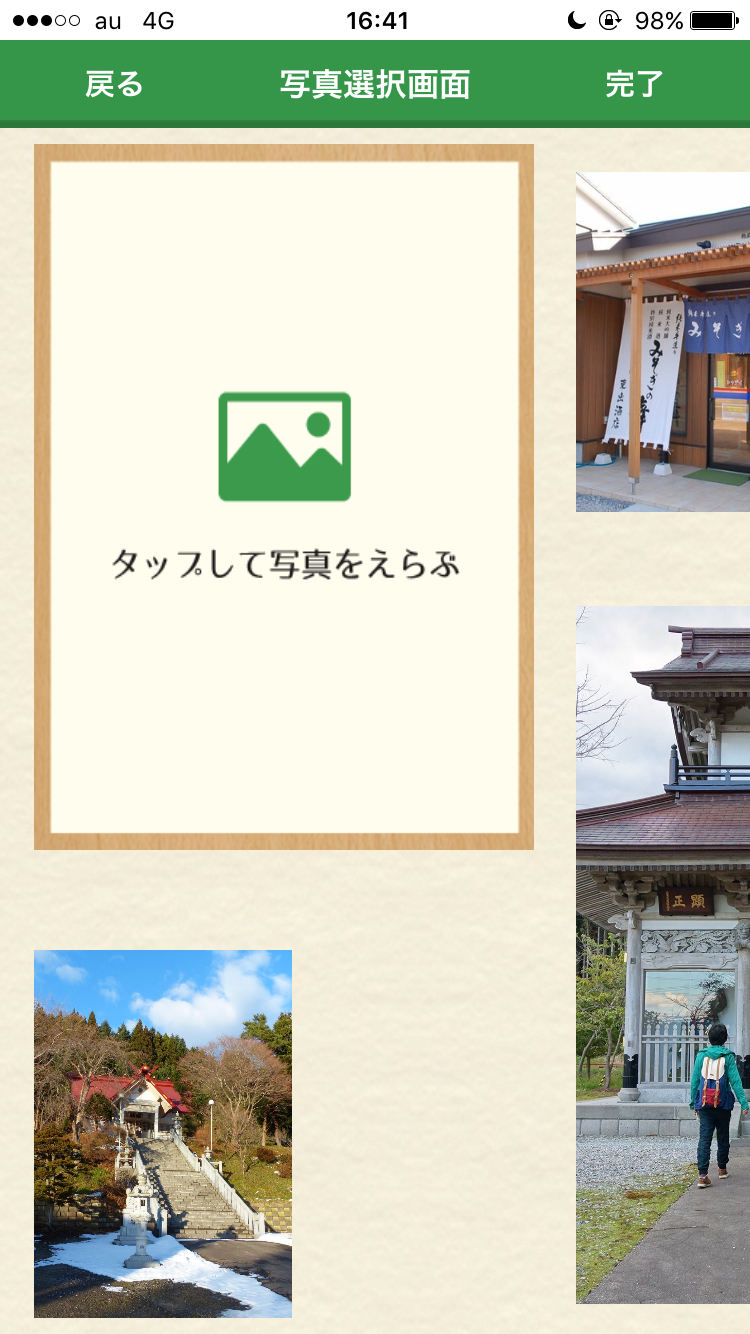
\includegraphics[width=4cm, bb=0 0 304 570]{kiko_print2.PNG}
          \hspace{1cm} (a)写真選択画面
        \end{center}
      \end{minipage}

      % 2
      \begin{minipage}{0.33\hsize}
        \begin{center}
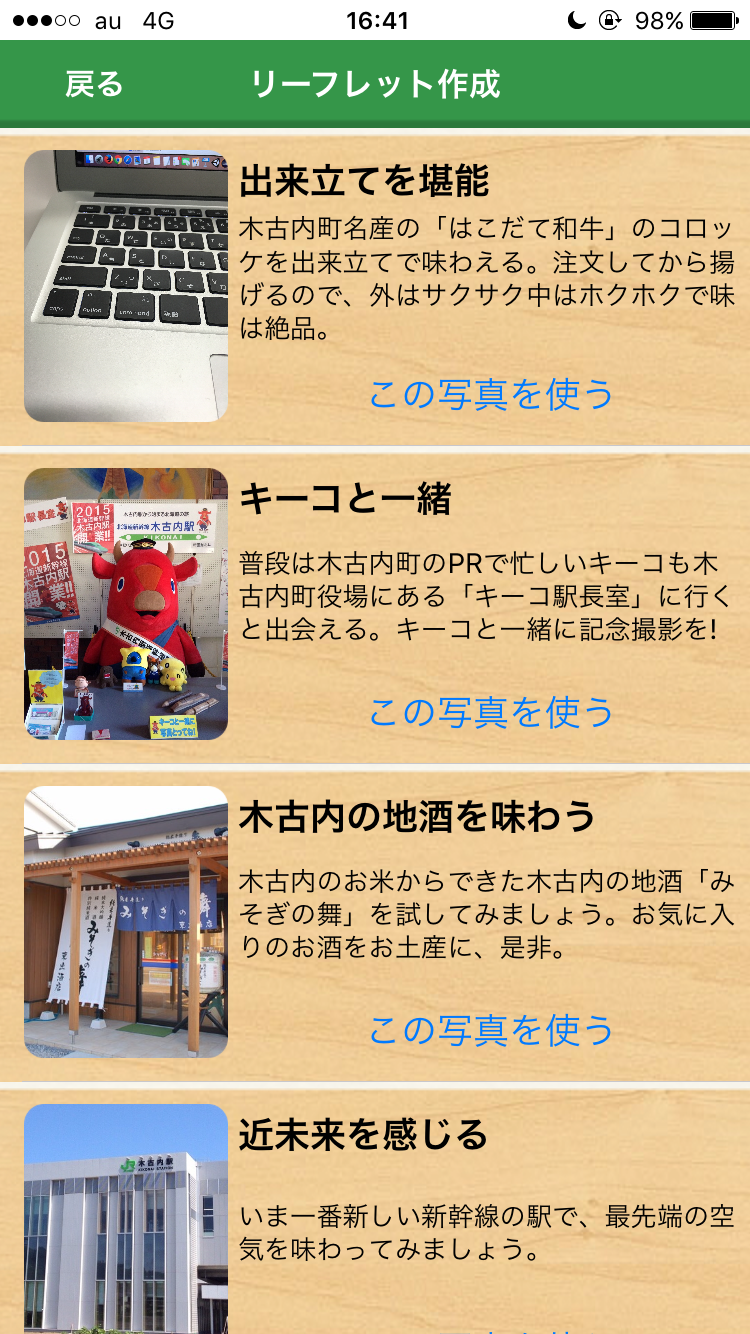
\includegraphics[width=4cm, bb=0 0 304 570]{kiko_print3.PNG}
          \hspace{1cm} (b)リーフレット作成画面
        \end{center}
      \end{minipage}
      
      \\
      
       % 3
      \begin{minipage}{0.33\hsize}
        \begin{center}
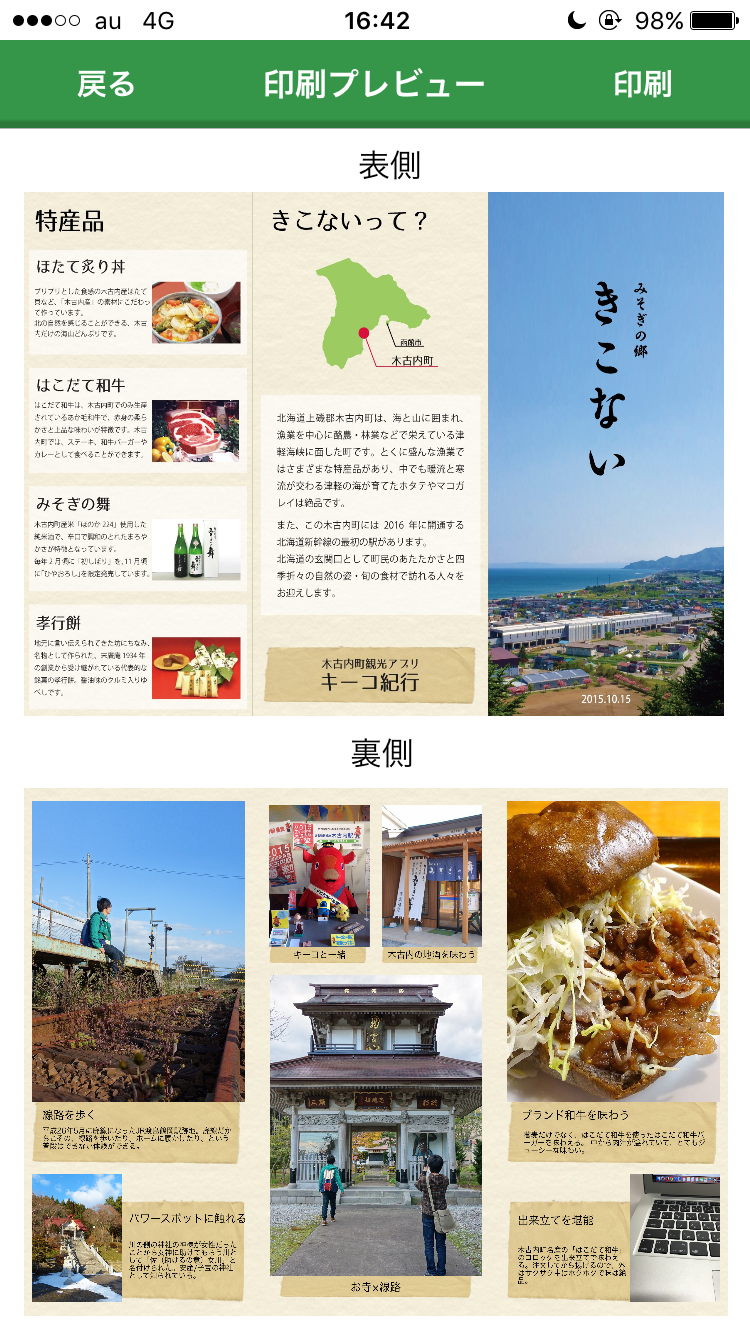
\includegraphics[width=4cm, bb=0 0 304 570]{kiko_print4.PNG}
          \hspace{1cm} (c)印刷プレビュー画面
        \end{center}
      \end{minipage}

      % 4
      \begin{minipage}{0.33\hsize}
        \begin{center}
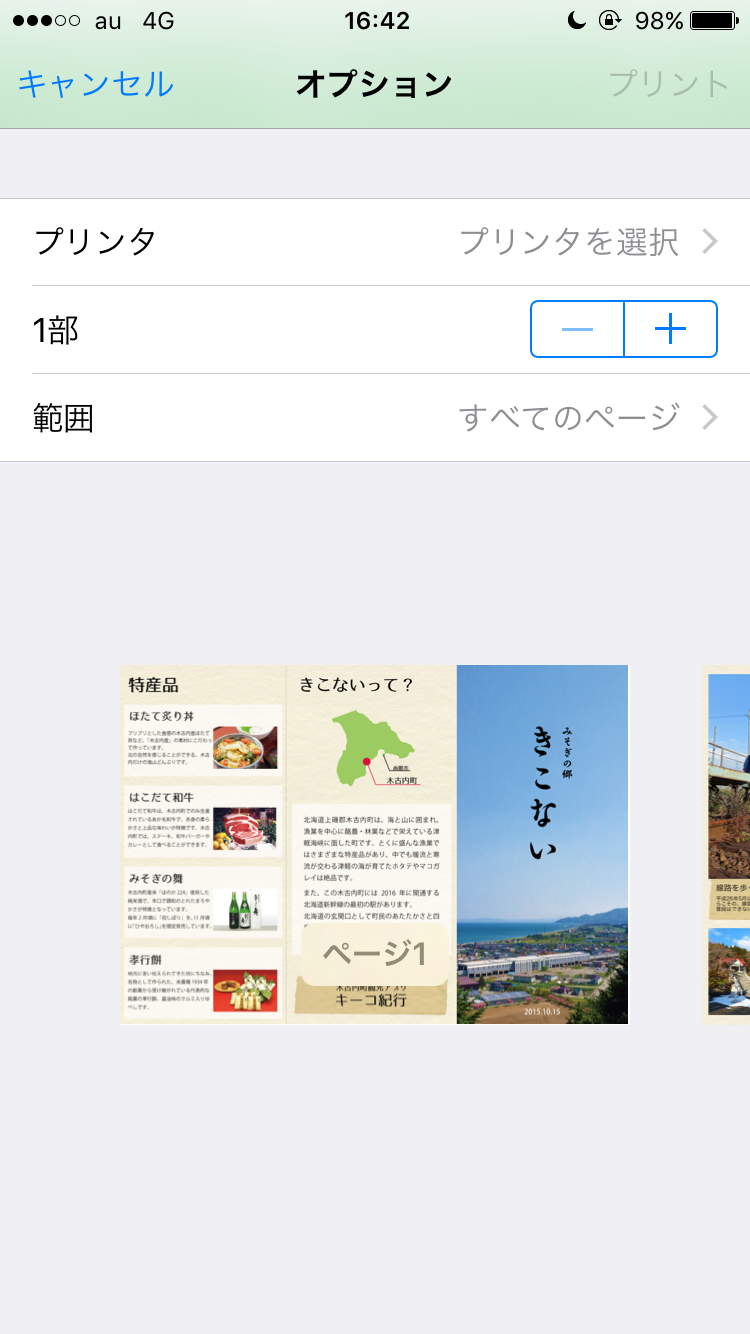
\includegraphics[width=4cm, bb=0 0 304 570]{kiko_print5.PNG}
          \hspace{1cm} (d)AirPrintの設定画面
        \end{center}
      \end{minipage}
      

    \end{tabular}
    \caption{印刷機能の画面}
    \label{fig:lena}
  \end{center}
\end{figure}       

\bunseki{池田俊輝}